\documentclass[../main.tex]{subfiles}
\begin{document}
\subsection{Introduzione}
Una funzione $f$ è una legge che associa ad ogni elemento $x$ di un insieme di partenza $A$ un \textbf{unico} elemento $y$ di un insieme di arrivo $B$.
\begin{center}
    \begin{tikzpicture}
        %sets A and B
        \draw (0,0) ellipse (1 and 2);
        \draw (5,0) ellipse (1 and 2);
        \node at (0, 2.3) {$A$};
        \node at (5,2.3) {$B$};
        \node at (2.5,0.3) {$f$};
        
        %set A
        \node at (0,0) {$\bullet$};
        \node at (-0.2,0.2) {$x$};

        
        %set B
        \node at (5,0) {$\bullet$};
        \node at (5.2,0.2) {$y$};
        
        %arrows
        \draw[->] (0.2,0) -- (4.8,0);
    \end{tikzpicture}
    \begin{align*}
        f:A& \longrightarrow B \\
        x& \longmapsto y = f(x)
    \end{align*}
\end{center}
$x$ è detto elemento di $A$ associato a $y$, elemento di $B$. \\

\subsubsection{Esempi}
\begin{enumerate}
    \item \begin{align*}
        f: \mathbb{R}& \longrightarrow \mathbb{R} \\
        x& \longmapsto y=3x-2 \\
        x&=5 \Rightarrow y=3\cdot5-2=13 \\
        &\Rightarrow f \text{ è una funzione}
    \end{align*}
    \item \begin{align*}
        f: \mathbb{R}& \longrightarrow \mathbb{R} \\
        x& \longmapsto y=\sqrt{x} \\
        x&=4 \Rightarrow y=\sqrt{4}=2 \\
        x&=-4 \Rightarrow y=\sqrt{-4} \\
        &\sqrt{-4} \text{ non esiste in } \mathbb{R} \\
        &\Rightarrow f \text{ non è una funzione}
    \end{align*}
    \item \begin{align*}
        f: \mathbb{R}& \longrightarrow \mathbb{R} \\
        x& \longmapsto y=\pm x^2 \\
        x&=3 \Rightarrow y=\pm 3^2=\pm 9 \\
        x&=+9 \\
        x&=-9 \\
    \end{align*}
    L'argomento possiede due immagini, $f$ \textbf{non} è una funzione
\end{enumerate}

\pagebreak
\subsection{Dominio}
Sia $f$ una funzione. Il suo dominio $D(f)$ è l'insieme di tutti gli elementi $x$ per i quali $f(x)$ è ben definita.

\subsubsection{Esempi}
\begin{enumerate}
    \item \begin{align*}
        f:D(&f) \rightarrow \mathbb{R} \\
        &x \mapsto f(x)=1/x \\
        D(&f)= \mathbb{R} \backslash \{0\}
    \end{align*}
    \item \begin{align*}
        f:D(&f) \rightarrow \mathbb{R} \\
        &x \mapsto y=\sqrt{x+2} \Rightarrow D(f)=\lbrack -2;+ \infty \lbrack
    \end{align*}
    \item \begin{align*}
        f:D(&f) \rightarrow \mathbb{R} \\
        &x \mapsto \frac{1}{\sqrt{x+2}} \Rightarrow D(f)= \rbrack -2;+\infty \lbrack
    \end{align*}
    \item \begin{align*}
        f:D(&f) \rightarrow \mathbb{R} \\
        &x \mapsto y=3x-1 \Rightarrow D(f)= \mathbb{R}
    \end{align*}
\end{enumerate}

\textbf{Nota:} il dominio è l'insieme di partenza più grande possibile, per trovarlo occorre innanzitutto analizzare le limitazioni della funzione, escludere i valori non validi e riportare l'insieme più grande possibile che non comprenda quei valori.
\begin{center}
    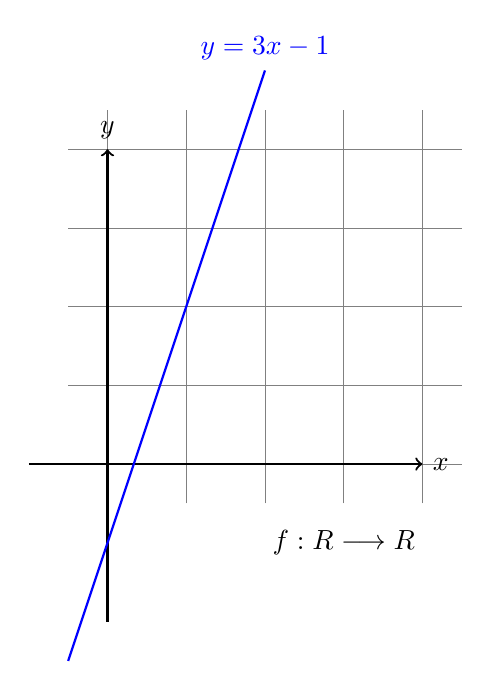
\begin{tikzpicture}
        % Disegna la griglia
        \draw[very thin, gray] (-0.5,-0.5) grid (4.5,4.5);
        
        % Disegna assi
        \draw[thick,->] (-1,0) -- (4,0) node[right] {$x$}; % Asse x
        \draw[thick,->] (0,-2) -- (0,4) node[above] {$y$}; % Asse y

        % Disegna la funzione y = 3x - 2
        \draw[domain=-0.5:2,smooth,variable=\x,blue,thick] 
        plot ({\x},{3*\x-1}) node[above] {$y = 3x - 1$};

        \node at (3, -1) {$f:\mathbb{R}\longrightarrow \mathbb{R}$};
    \end{tikzpicture} \hspace{2cm}
    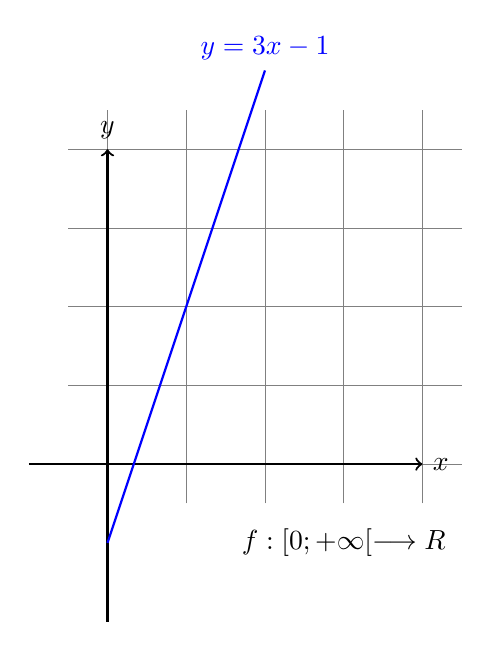
\begin{tikzpicture}
        % Disegna la griglia
        \draw[very thin, gray] (-0.5,-0.5) grid (4.5,4.5);
        
        % Disegna assi
        \draw[thick,->] (-1,0) -- (4,0) node[right] {$x$}; % Asse x
        \draw[thick,->] (0,-2) -- (0,4) node[above] {$y$}; % Asse y

        % Disegna la funzione y = 3x - 2
        \draw[domain=0:2,smooth,variable=\x,blue,thick] 
        plot ({\x},{3*\x-1}) node[above] {$y = 3x - 1$};

        \node at (3, -1) {$f:\lbrack 0; +\infty \lbrack \longrightarrow \mathbb{R}$};
    \end{tikzpicture}
\end{center}

\pagebreak
\subsection{Insieme immagini}
Sia $f:A \rightarrow B$ una funzione. Il suo insieme delle immagini è definito come segue:
$$
    Im(f)= \{ y=f(x)|x \in A \}
$$
Generalmente $x$ indica gli argomenti e $y$ le immagini, nello schema visto nell'introduzione $B$
rappresenta l'insieme delle immagini. Tutti gli elementi di $A$ sono associati ad un elemento di $B$,
ma non per forza viceversa.

\subsubsection{Esempi}
\begin{align*}
    f: \mathbb{R}& \longrightarrow \mathbb{R} \\
    x& \longmapsto y=3x-1 \\
    &\Rightarrow Im(f)=\mathbb{R}
\end{align*}
In questo caso per trovare $Im$ guardiamo il grafico.

\begin{center}
    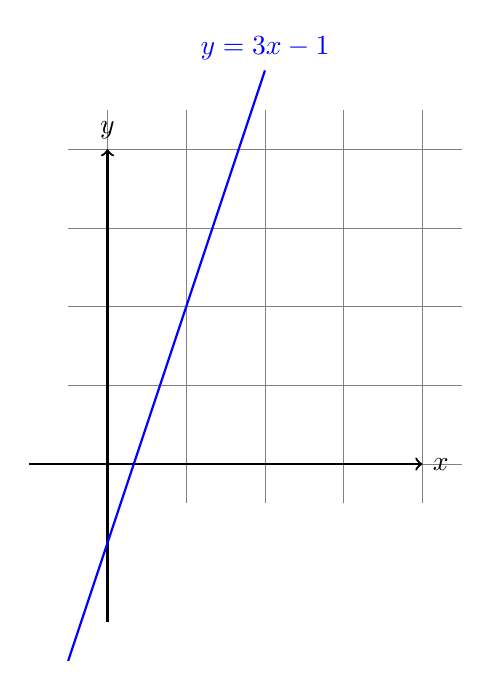
\begin{tikzpicture}
        % Disegna la griglia
        \draw[very thin, gray] (-0.5,-0.5) grid (4.5,4.5);
        
        % Disegna assi
        \draw[thick,->] (-1,0) -- (4,0) node[right] {$x$}; % Asse x
        \draw[thick,->] (0,-2) -- (0,4) node[above] {$y$}; % Asse y

        % Disegna la funzione y = 3x - 2
        \draw[domain=-0.5:2,smooth,variable=\x,blue,thick] 
        plot ({\x},{3*\x-1}) node[above] {$y = 3x - 1$};
    \end{tikzpicture}
\end{center}

\begin{align*}
    g: \mathbb{R}& \longrightarrow \mathbb{R} \\
    x& \longmapsto x^2-2 \\
    &\Rightarrow Im(g)= \lbrack -2; + \infty \lbrack \\
    &= \lbrack y_v;+ \infty \lbrack
\end{align*}
In questo caso trattandosi di una \textbf{parabola}, per determinare $Im(g)$ guardiamo il vertice.

\textbf{Nota:} Non esiste una ricetta o una procedura precisa per trovare l'$Im$ di una funzione, non è come per il dominio.

\pagebreak
\subsection{Grafico di una funzione}
Sia $f:A \rightarrow B$ una funzione. Il suo grafico $G(f)$ è l'insieme dei punti 
$$
    G(f)= \{ (a;f(a)) | a \in A \}
$$

\begin{tikzpicture}[x=0.75pt,y=0.75pt,yscale=-1,xscale=1]
    %uncomment if require: \path (0,300); %set diagram left start at 0, and has height of 300
    
    %Shape: Axis 2D [id:dp7439597163468655] 
    \draw  (60.68,251.63) -- (555.67,251.63)(110.17,137.25) -- (110.17,264.34) (548.67,246.63) -- (555.67,251.63) -- (548.67,256.63) (105.17,144.25) -- (110.17,137.25) -- (115.17,144.25)  ;
    %Straight Lines [id:da7977119812178095] 
    \draw [color={rgb, 255:red, 251; green, 0; blue, 0 }  ,draw opacity=1 ][line width=0.75]  [dash pattern={on 0.84pt off 2.51pt}]  (329.55,156.86) -- (329.83,252) ;
    %Straight Lines [id:da6782457373660774] 
    \draw [color={rgb, 255:red, 251; green, 0; blue, 0 }  ,draw opacity=1 ][line width=0.75]  [dash pattern={on 0.84pt off 2.51pt}]  (329.55,156.86) -- (313.94,156.78) -- (110,156.25) ;
    %Shape: Ellipse [id:dp1285941766712374] 
    \draw  [color={rgb, 255:red, 247; green, 2; blue, 2 }  ,draw opacity=1 ][fill={rgb, 255:red, 252; green, 5; blue, 5 }  ,fill opacity=1 ] (325.11,155.34) .. controls (325.11,153.23) and (326.73,151.52) .. (328.72,151.52) .. controls (330.72,151.52) and (332.33,153.23) .. (332.33,155.34) .. controls (332.33,157.45) and (330.72,159.17) .. (328.72,159.17) .. controls (326.73,159.17) and (325.11,157.45) .. (325.11,155.34) -- cycle ;
    %Curve Lines [id:da9750121639766473] 
    \draw [color={rgb, 255:red, 74; green, 144; blue, 226 }  ,draw opacity=1 ]   (74.37,251.93) .. controls (90.56,239.78) and (141.2,201.43) .. (175.37,207.93) .. controls (209.53,214.43) and (224.7,286.38) .. (256.37,269.93) .. controls (283.63,255.77) and (299.52,165.2) .. (325.11,156.86) .. controls (329.25,155.51) and (333.63,156.31) .. (338.37,159.93) .. controls (372.37,185.93) and (391.16,255.4) .. (440.37,267.93) .. controls (489.57,280.46) and (546.79,183.04) .. (547.37,177.93) ;
    
    % Text Node
    \draw (45.98,153.1) node [anchor=north west][inner sep=0.75pt]    {$\textcolor[rgb]{0.94,0.02,0.02}{b=f}\textcolor[rgb]{0.94,0.02,0.02}{(}\textcolor[rgb]{0.94,0.02,0.02}{a}\textcolor[rgb]{0.94,0.02,0.02}{)}$};
    % Text Node
    \draw (320.91,131.24) node [anchor=north west][inner sep=0.75pt]    {$\textcolor[rgb]{0.98,0.04,0.04}{(}\textcolor[rgb]{0.98,0.04,0.04}{a;b}\textcolor[rgb]{0.98,0.04,0.04}{)}$};
    % Text Node
    \draw (325.14,253.54) node [anchor=north west][inner sep=0.75pt]    {$\textcolor[rgb]{0.95,0.02,0.02}{a}$};
\end{tikzpicture}

$(a;b) \in G(f) \Leftrightarrow b = f(a)$, Un punto appartiene al grafico se e solo se $b=f(a)$


\textbf{Osservazione:}
\begin{center}
    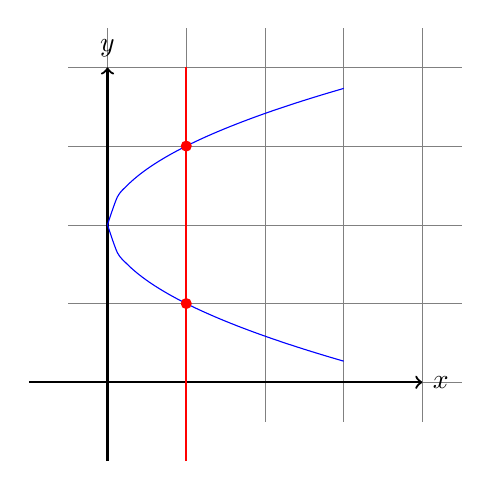
\begin{tikzpicture}
        % Disegna la griglia
        \draw[very thin, gray] (-0.5,-0.5) grid (4.5,4.5);
        
        % Disegna assi
        \draw[thick,->] (-1,0) -- (4,0) node[right] {$x$}; % Asse x
        \draw[thick,->] (0,-1) -- (0,4) node[above] {$y$}; % Asse y

        \draw[domain=0:3,smooth,variable=\x,blue] plot ({\x},{sqrt(\x) + 2});
        \draw[domain=0:3,smooth,variable=\x,blue] plot ({\x},{-sqrt(\x) + 2});

        \draw[red, thick] (1,-1) -- (1,4);  % Linea tratteggiata a x = 1

        \fill[red] (1, 1) circle (2pt);  % Punto a (1, 1) con raggio di 5pt
        \fill[red] (1, 3) circle (2pt);  % Punto a (1, 1) con raggio di 5pt
    \end{tikzpicture} \hspace{2cm}
\end{center}
Questo grafico non rappresenta una funzione, per alcuni argomenti ci sono più immagini.

\pagebreak
\subsection{Operazioni con le funzioni}
\subsubsection{Somma - Sottrazione}
Esempio:
\begin{align*}
    f(x)&=\sqrt{x+1} \Rightarrow D(f)=\lbrack-1;+\infty\lbrack \\
    g(x)&=\frac{1}{x}\Rightarrow D(g)=\mathbb{R} \backslash \{0\} \\
    (f\pm g)(x)&=\sqrt{x+1}\pm \frac{1}{x} \\
    \Rightarrow D(f+g)&=\lbrack-1;+\infty\lbrack \backslash \{0\} \\
    &=D(f)\cap D(g)
\end{align*}
\begin{center}
    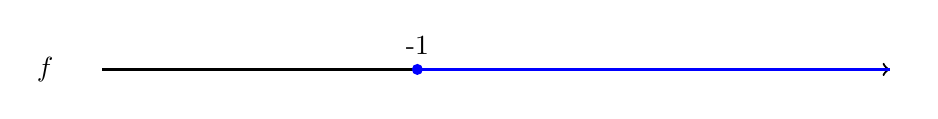
\begin{tikzpicture}        
        % Disegna assi
        \draw[thick,->] (-5,0) -- (5,0) node[right] {}; % Asse x

        \node at (-5.5, 0) {$f\phantom{+g}$};

        \node at (-1, 0.3) {-1};
        \fill[blue] (-1, 0) circle (2pt);  % Punto a (1, 1) con raggio di 5pt

        % Disegna la parte colorata in blu
        \draw[blue, thick] (-1, 0) -- (5, 0); % Parte blu della retta
    \end{tikzpicture}
\end{center}
\begin{center}
    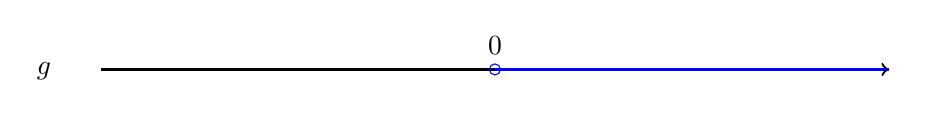
\begin{tikzpicture}        
        % Disegna assi
        \draw[thick,->] (-5,0) -- (5,0) node[right] {}; % Asse x

        \node at (-5.5, 0) {$g\phantom{+g}$};

        \node at (0, 0.3) {0};
        \draw[blue] (0, 0) circle (2pt);  % Punto a (1, 1) con raggio di 5pt

        % Disegna la parte colorata in blu
        \draw[blue, thick] (0, 0) -- (5, 0); % Parte blu della retta
    \end{tikzpicture}
\end{center}
\begin{center}
    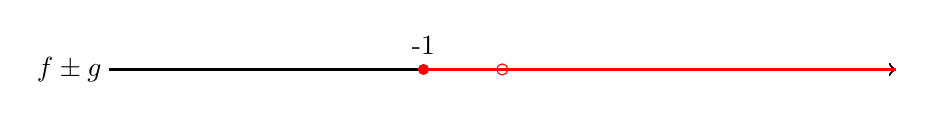
\begin{tikzpicture}        
        % Disegna assi
        \draw[thick,->] (-5,0) -- (5,0) node[right] {}; % Asse x

        \node at (-5.5, 0) {$f\pm g$};

        \node at (-1, 0.3) {-1};
        \fill[red] (-1, 0) circle (2pt);  % Punto a (1, 1) con raggio di 5pt
        \draw[red] (0, 0) circle (2pt);  % Punto a (1, 1) con raggio di 5pt

        % Disegna la parte colorata in blu
        \draw[red, thick] (-1, 0) -- (5, 0); % Parte blu della retta
    \end{tikzpicture}
\end{center}

In generale
\begin{align*}
    (f\pm g)(x) = f(x)\pm g(x)\\
    D(f\pm g) = D(f) \cap D(g) 
\end{align*}

\subsubsection{Prodotto}
Esempio:
\begin{align*}
    f(x) = \sqrt{x + 1} \Rightarrow& D(f) = [-1; +\infty[ \\
    g(x) = x \Rightarrow& D(g) = \mathbb{R} \\
    \Rightarrow (f \cdot g)(x) =& x \cdot \sqrt{x + 1} \\
    \Rightarrow D(f \cdot g) =& [-1;+\infty[
\end{align*}

In generale
\begin{align*}
    (f \cdot g)(x) = f(x) \cdot g(x) \\
    D(f \cdot g) = D(f) \cap D(g)  
\end{align*}

\subsubsection{Divisione}
Esempio:
\begin{align*}
    f(x) = \frac{1}{x} \Rightarrow& D(f) = \mathbb{R}^* \\
    g(x) = \sqrt{x + 2} \Rightarrow& D(g) = [-2;+\infty[ \\
    \Rightarrow \frac{f}{g}(x) =& \frac{1/x}{\sqrt{x + 2}} = \frac{1}{x \cdot \sqrt{x + 2}} \\
    D(\frac{f}{g}) =& \color{red}]\color{black}-2;+\infty[\backslash \{0\}
\end{align*}

In generale
\begin{align*}
    (\frac{f}{g})(x) =& \frac{f(x)}{g(x)} \\
    D(\frac{f}{g}) =& D(f) \cap D(g) \backslash \{x \in D(g) | g(x) = 0\}
\end{align*}
\textbf{Nota:} Il dominio non è dato solo dall'intersezione, nell'esempio sopra va anche escluso il -2 che non si può dividere per 0.

\subsubsection{Composizione di funzioni}
\begin{center}
    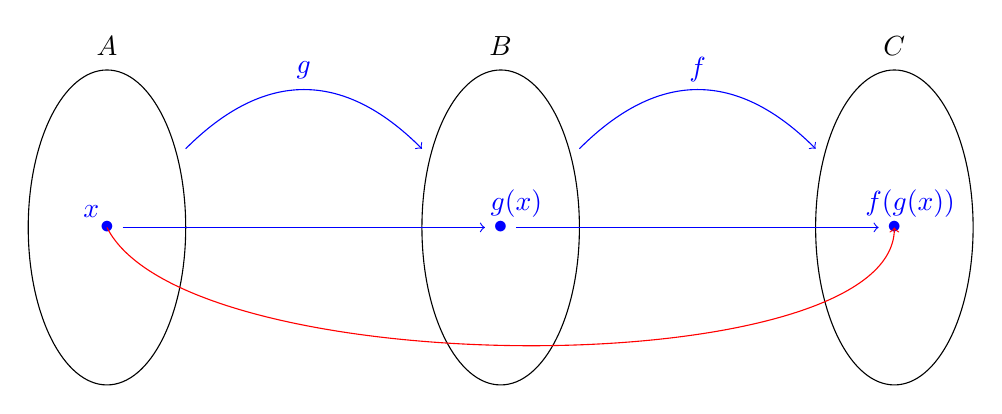
\begin{tikzpicture}
        %sets A and B
        \draw (-5,0) ellipse (1 and 2);
        \draw (0,0) ellipse (1 and 2);
        \draw (5,0) ellipse (1 and 2);
        \node at (-5, 2.3) {$A$};
        \node at (0,2.3) {$B$};
        \node at (5,2.3) {$C$};

        
        %set A
        \node at (-5,0) {\textcolor{blue}{$\bullet$}};
        \node at (-5.2, 0.2) {\textcolor{blue}{$x$}};
        
        %set B
        \node at (0,0) {\textcolor{blue}{$\bullet$}};
        \node at (0.2,0.3) {\textcolor{blue}{$g(x)$}};

        %set C
        \node at (5,0) {\textcolor{blue}{$\bullet$}};
        \node at (5.2,0.3) {\textcolor{blue}{$f(g(x))$}};
        
        %arrows
        \draw[->, blue] (-4.8,0) -- (-0.2,0);
        \draw[->, blue] (0.2,0) -- (4.8,0);

        \draw[->, blue] (-4, 1) .. controls (-3, 2) and (-2,2).. (-1, 1); % Freccia curva
        \node at (-2.5,2) {\textcolor{blue}{$g$}};
        \draw[->, blue] (1, 1) .. controls (2, 2) and (3,2).. (4, 1); % Freccia curva
        \node at (2.5,2) {\textcolor{blue}{$f$}};

        \draw[->, red] (-5, 0) .. controls (-4, -2) and (5,-2).. (5, 0); % Freccia curva
    \end{tikzpicture}
\end{center}

\vspace{1cm}
Date due funzioni
\begin{align*}
    f: B \longrightarrow& C \\
    g: A \longrightarrow& B \\
    \text{la funzione}
\end{align*}
la funzione
\begin{align*}
    f \circ  g: A \longrightarrow& C \\
    x \longrightarrow& (f \circ  g)(x) = f(g(x))
\end{align*}
è detta \textbf{composizione di f con g} ($f$ composto $g$).

\textbf{Nota:} In generale $f \circ g \neq g \circ  f $, la composizione di funzioni non è commutativa. 

\subsection{Funzione inversa}
Sia $f:A\rightarrow B$ una funzione

\end{document}